\documentclass[11pt, a4paper]{article}
%\usepackage{proj1}
\usepackage{natbib}
\usepackage{fancyhdr}  
\usepackage{subcaption}
\usepackage{caption}
\usepackage{graphicx}
\usepackage{numprint}
\usepackage{multirow}
\linespread{1.25} 
\setlength{\parindent}{0cm}
\graphicspath{{Images/}}
\usepackage{hyperref}
\usepackage{amsmath}
\usepackage{amsfonts}
\usepackage{amssymb}
\usepackage{amsthm}
\usepackage{mathtools}
\usepackage{commath}
\usepackage{bbm}

%\usepackage[sc,osf]{mathpazo}
\usepackage{subcaption}
\usepackage[a4paper, top=1in, left=1.0in, right=1.0in, bottom=1in, includehead, includefoot]{geometry} %Usually have top as 1in

\usepackage{listings}
\usepackage{color} %red, green, blue, yellow, cyan, magenta, black, white
\definecolor{mygreen}{RGB}{28,172,0} % color values Red, Green, Blue
\definecolor{mylilas}{RGB}{170,55,241}


\hypersetup{colorlinks,linkcolor={black},citecolor={blue},urlcolor={black}}
\usepackage{color}
\urlstyle{same}


\theoremstyle{definition}
\newtheorem{definition}{Definition}[section]

%\newcommand{\Sta}{\rho}
\newcommand{\adja}{q_a}
\newcommand{\adjb}{q_b}
\newcommand{\adjaB}{q_{a,\partial \Omega}}
\newcommand{\adjbB}{q_{b,\partial \Omega}}
%\newcommand{\Con}{u}
\newcommand{\ra}{\rho_a}
\newcommand{\rb}{\rho_b}
\newcommand{\w}{\mathbf{w}}
\newcommand{\Stav}{\mathbf{v}}
\newcommand{\Adja}{\mathbf{p}}
\newcommand{\Adjb}{q}
\newcommand{\Adjc}{{p}_{\partial \Sigma}}
\newcommand{\Con}{\mathbf{f}}
\newcommand{\n}{\mathbf{n}}
\newcommand{\h}{\mathbf{h}}
\newcommand{\K}{\mathbf{K}}


\pagenumbering{gobble}
\begin{document}
	



\section*{Periodic Sedimentation}

I scaled the equation with time $t^* = t/ \tau_B$, where $\tau_B = \beta \sigma^2/ \Gamma$.
We have:
\begin{align*}
	\frac{\partial \rho}{\partial t} = \Gamma \nabla \left(\rho \nabla \frac{\delta F[\rho]}{\delta \rho}\right)
\end{align*}
and so
\begin{align*}
	\frac{\partial \rho}{\partial t^*} &= \Gamma \tau_B \nabla \left(\rho \nabla \frac{\delta F[\rho]}{\delta \rho}\right)\\
	& = \beta \sigma^2 \nabla \left(\rho \nabla \frac{\delta F[\rho]}{\delta \rho}\right).
\end{align*}
Since we set $\beta = 1$, I have scaled the equation in the code by $\sigma^2$.
Choosing $\sigma = 1$, $\bar \rho = 0.072$, $\epsilon = 3.5$ and $a =0.1$, where the only choice I made is $\sigma$, the rest is determined by the paper. I checked before that the points are random and they are and the interval is $\bar \rho \pm \frac{1}{20}$. Then I let this run up to $t^* = 300$, like in the paper.
\begin{figure}[h]
	\centering
	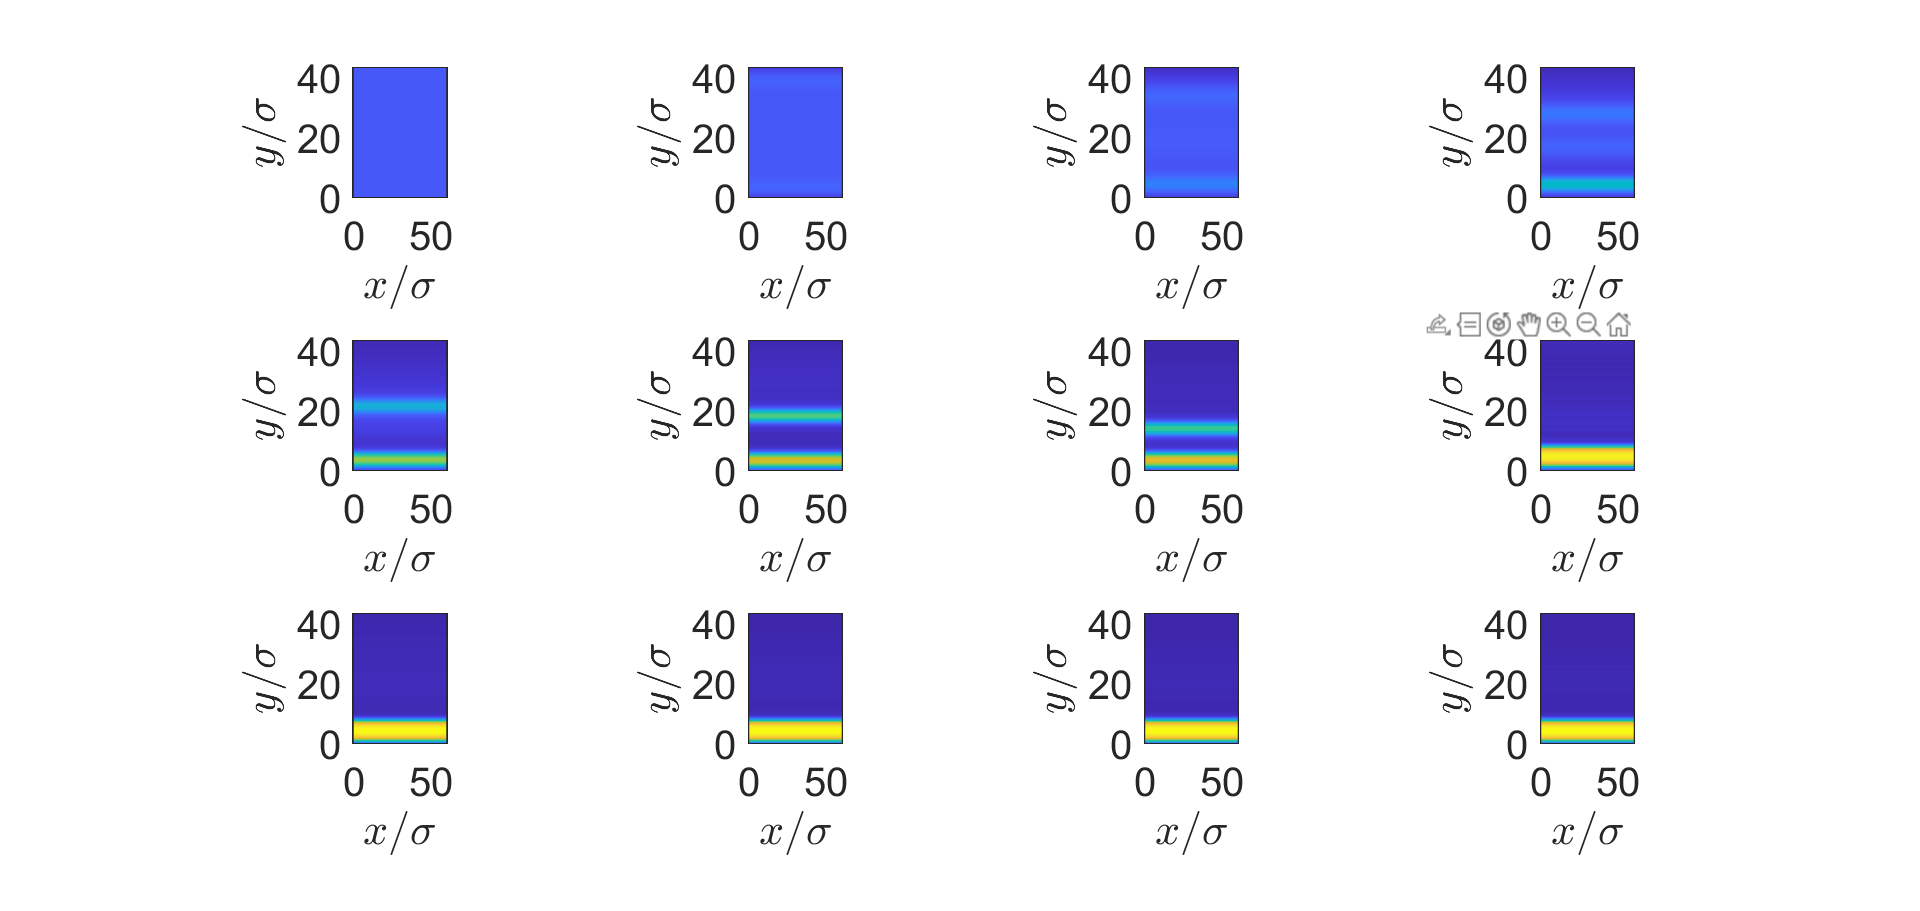
\includegraphics[scale=0.4]{Sed1.png}
	\caption{Figure 8 from paper with $\sigma = 1$.} 
	\label{F1}
\end{figure}
Then I chose the initial condition with more randomness: $\bar \rho \pm \frac{1}{10}$.
\begin{figure}[h]
	\centering
	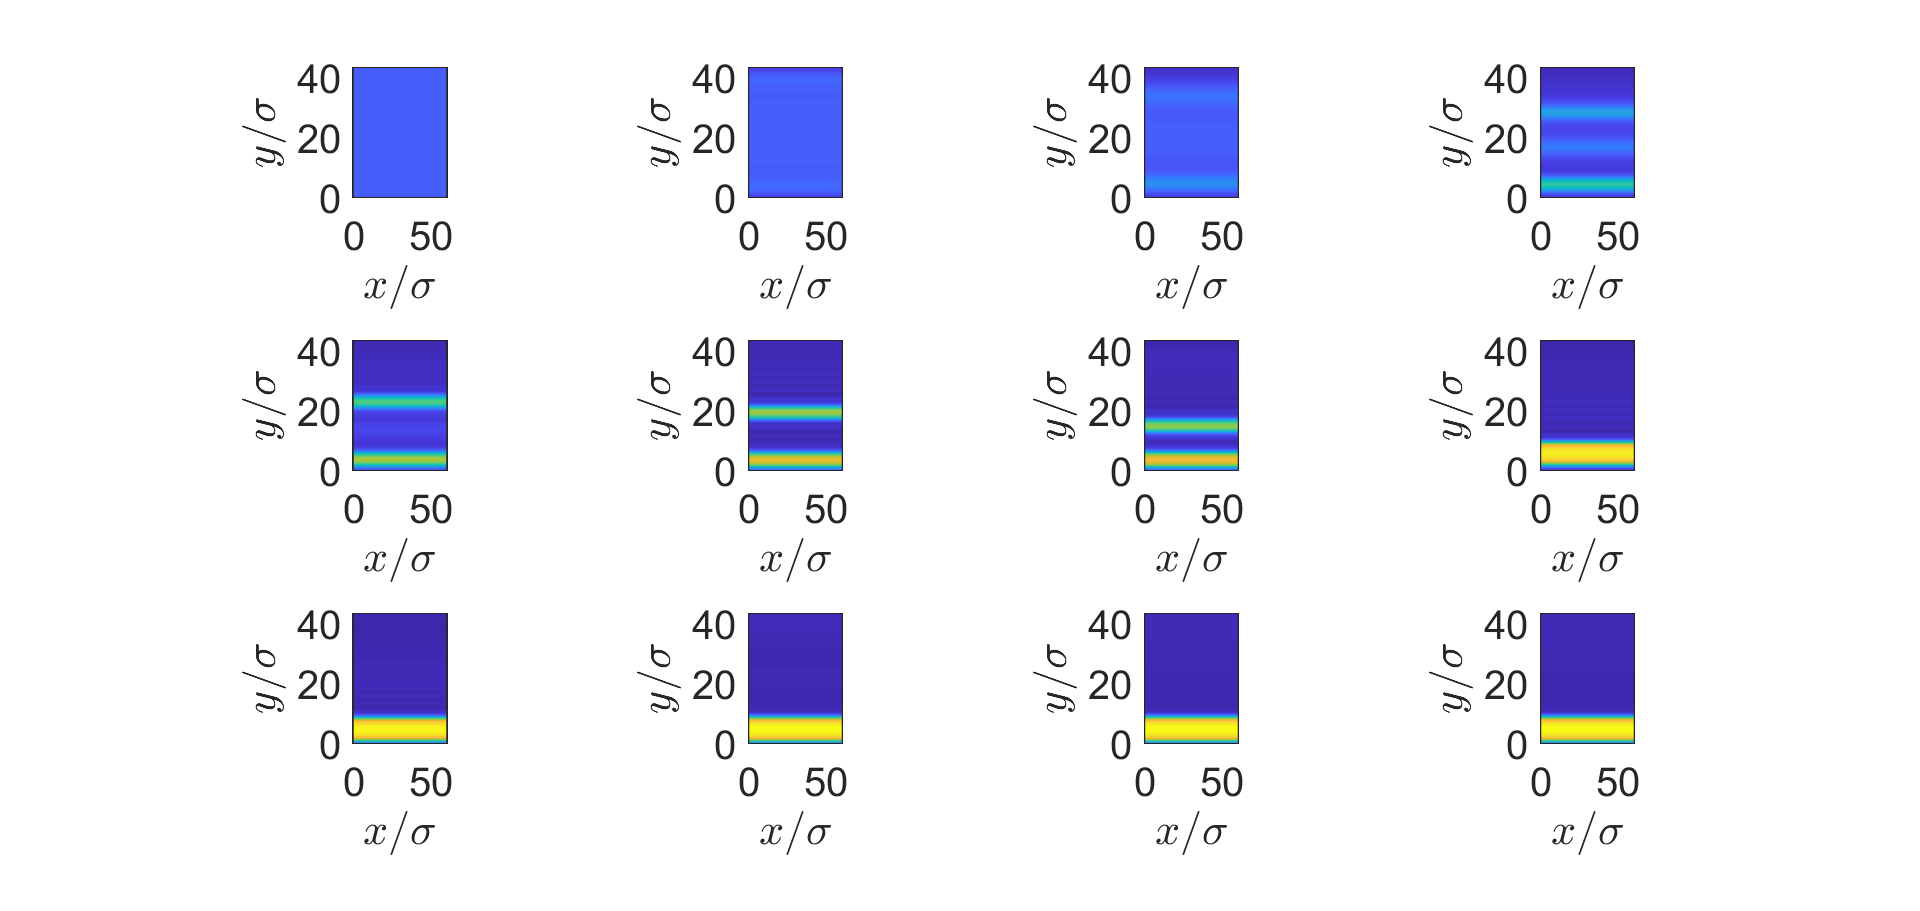
\includegraphics[scale=0.4]{Sed2.png}
	\caption{Figure 8 from paper with $\sigma = 1$, more randomness in $\rho_0$.} 
	\label{F1a}
\end{figure}

Then I chose $\bar \rho = 0.072 (\cos(\pi y_2/15) +1 )$, to see what happens if there are already clusters in the initial condition.


\begin{figure}[h]
	\centering
	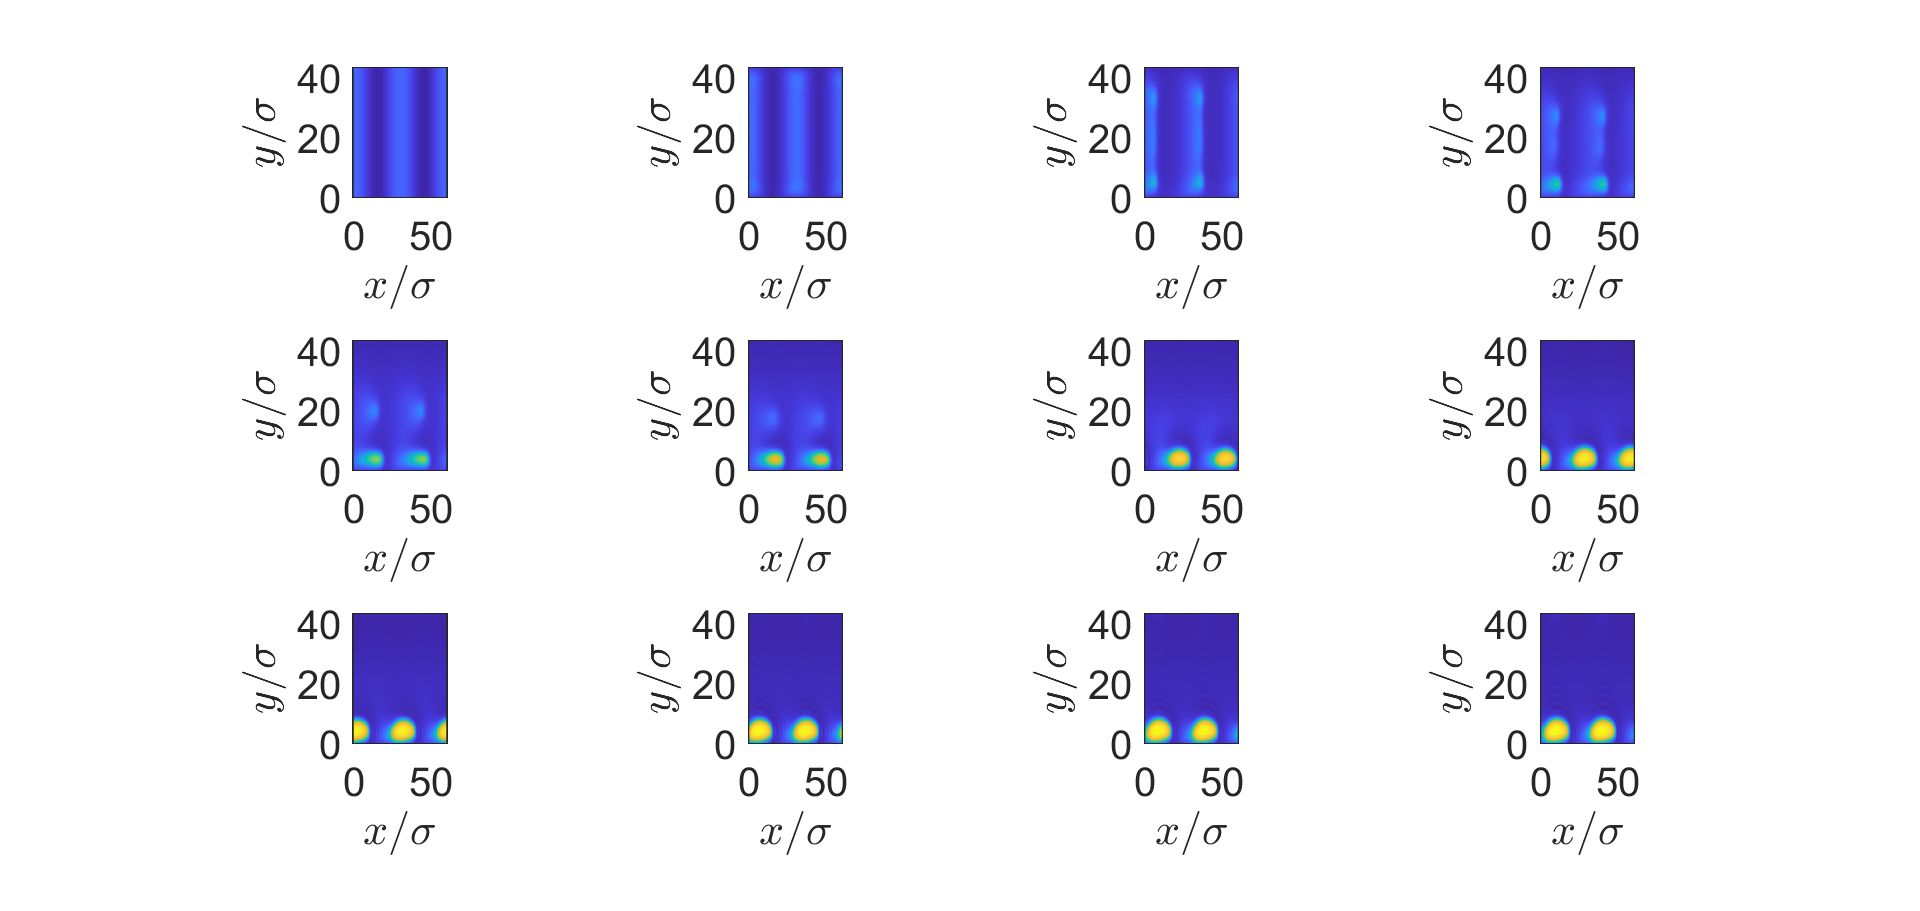
\includegraphics[scale=0.4]{Sed3.png}
	\caption{Figure 8 from paper with $\sigma = 1$, $\bar \rho = 0.072 (\cos(\pi y_2/15) +1 )$.} 
	\label{F1b}
\end{figure}

Then I chose $\bar \rho = 0.072 (\cos(\pi y_2/5) +1 )$, to see what happens if there are already clusters in the initial condition.


\begin{figure}[h]
	\centering
	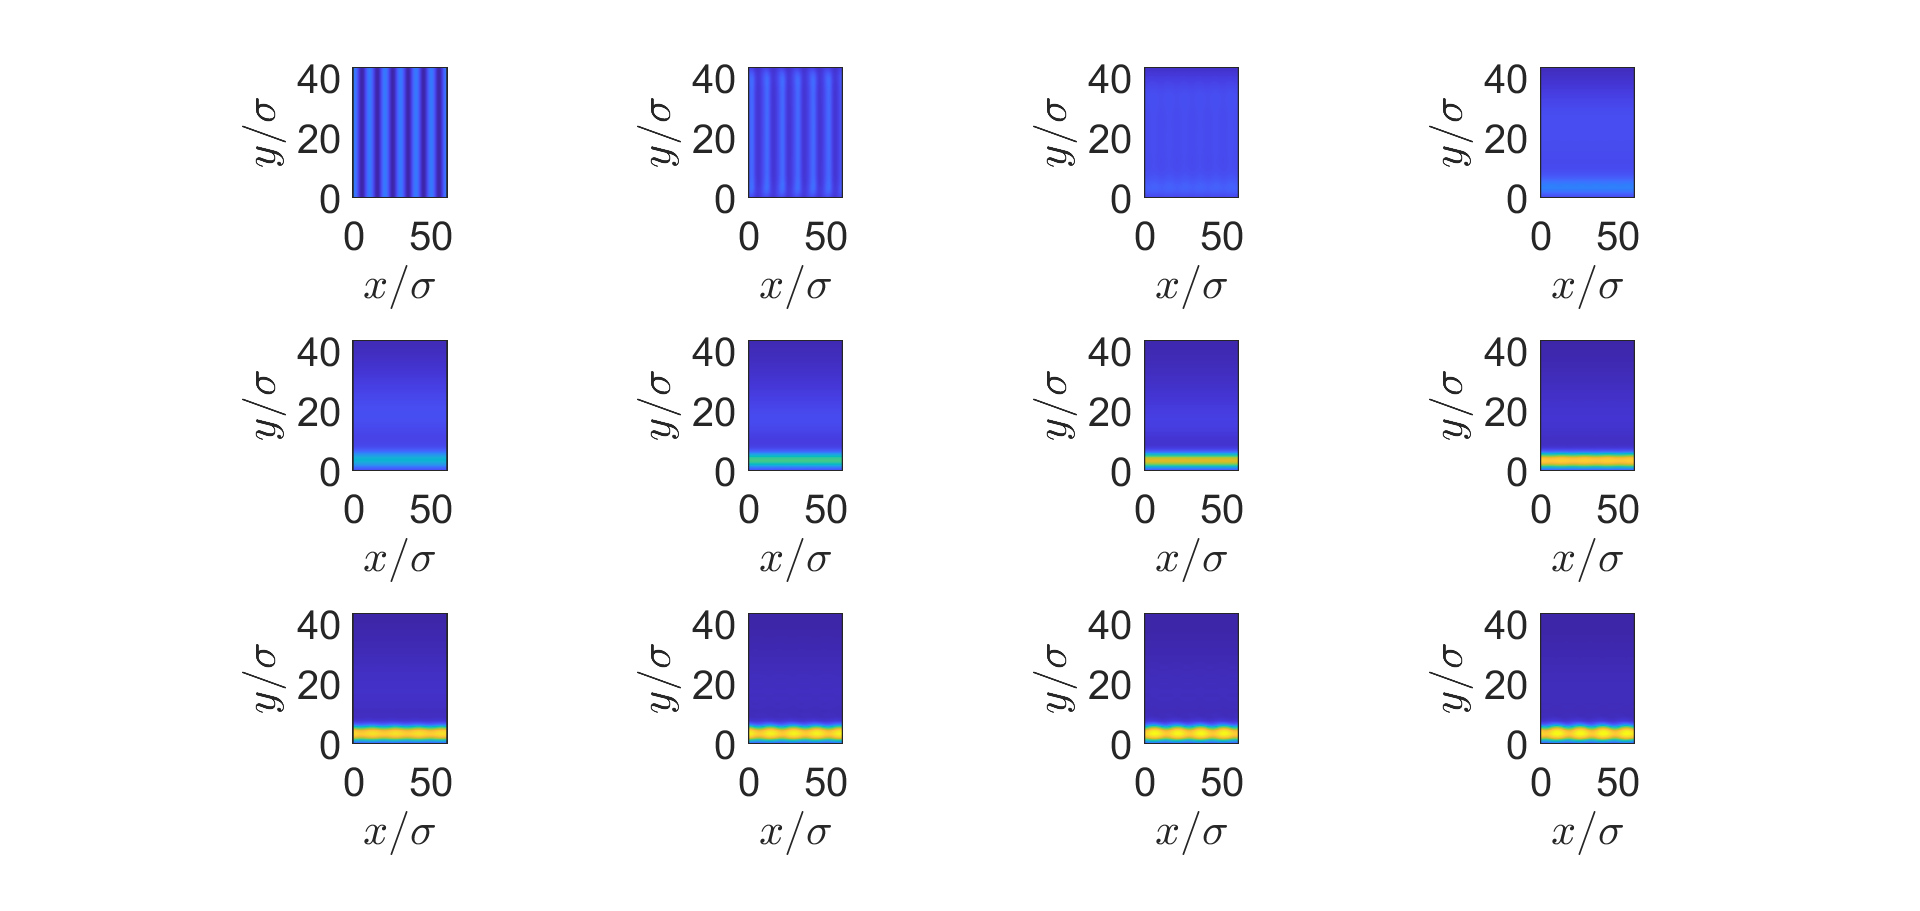
\includegraphics[scale=0.4]{Sed4.png}
	\caption{Figure 8 from paper with $\sigma = 1$, $\bar \rho = 0.072 (\cos(\pi y_2/5) +1 )$.} 
	\label{F1c}
\end{figure}
\begin{figure}[h]
	\centering
	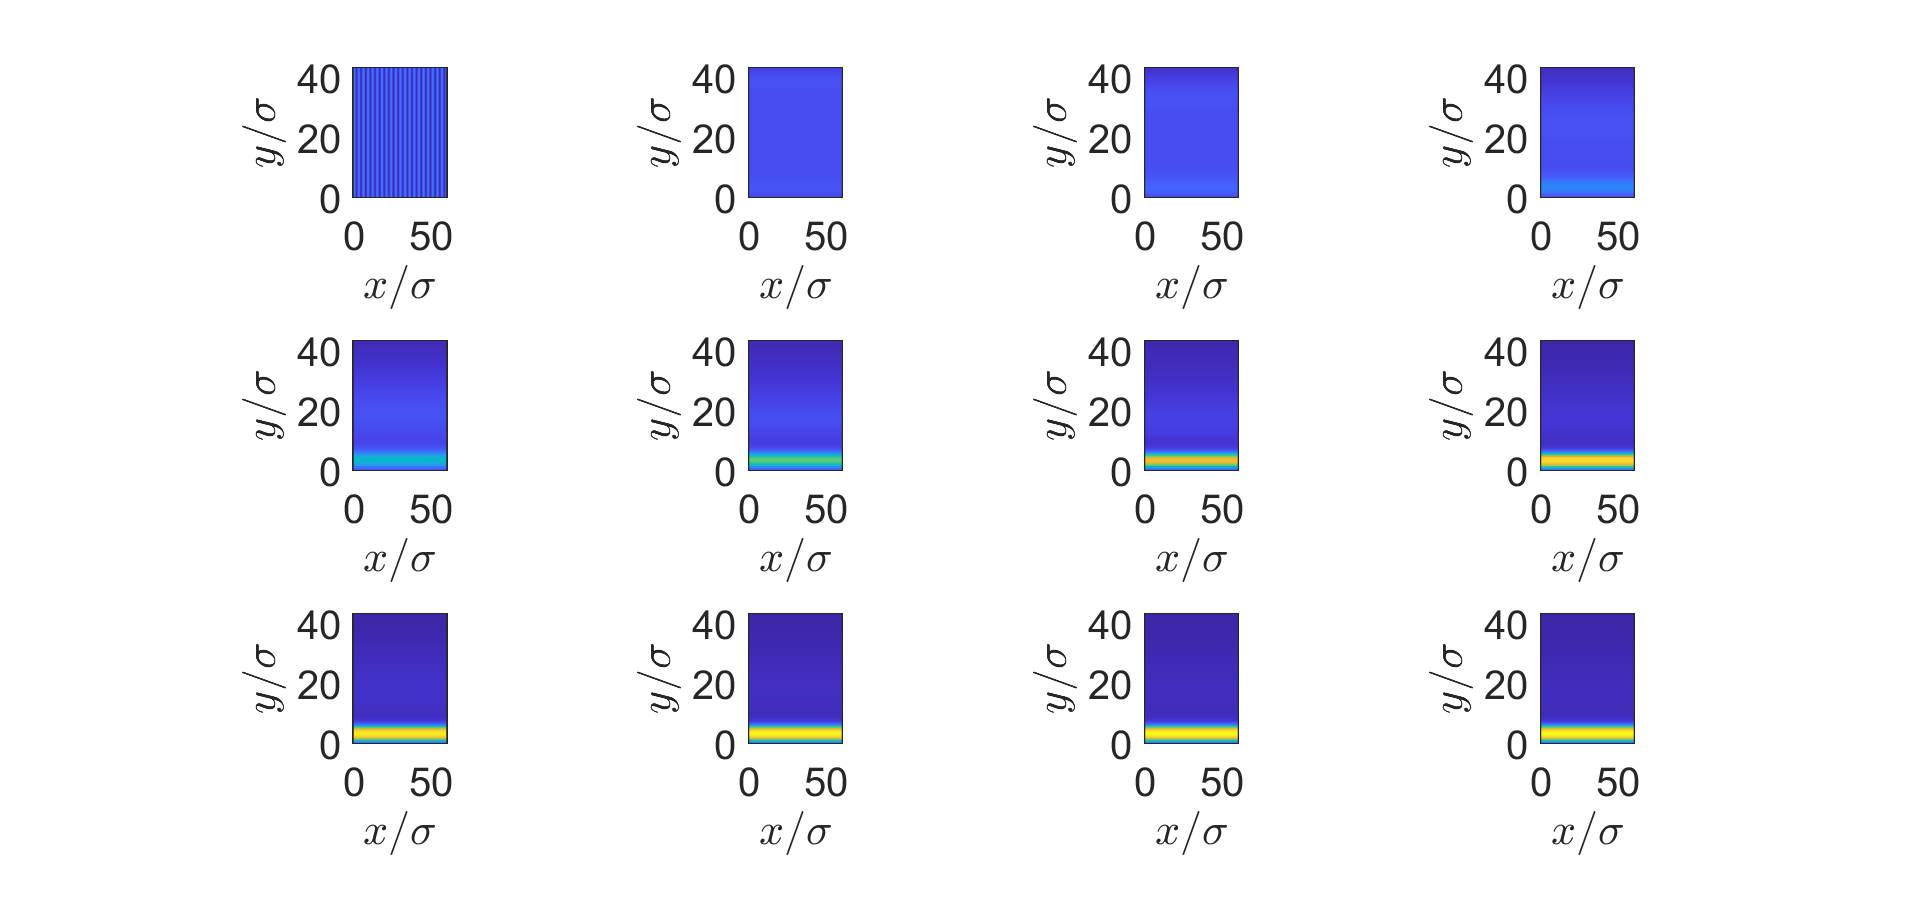
\includegraphics[scale=0.4]{Sed5.png}
	\caption{Figure 8 from paper with $\sigma = 1$, $\bar \rho = 0.072 (\cos(\pi y_2) +1 )$.} 
	\label{F1d}
\end{figure}
\begin{figure}[h]
	\centering
	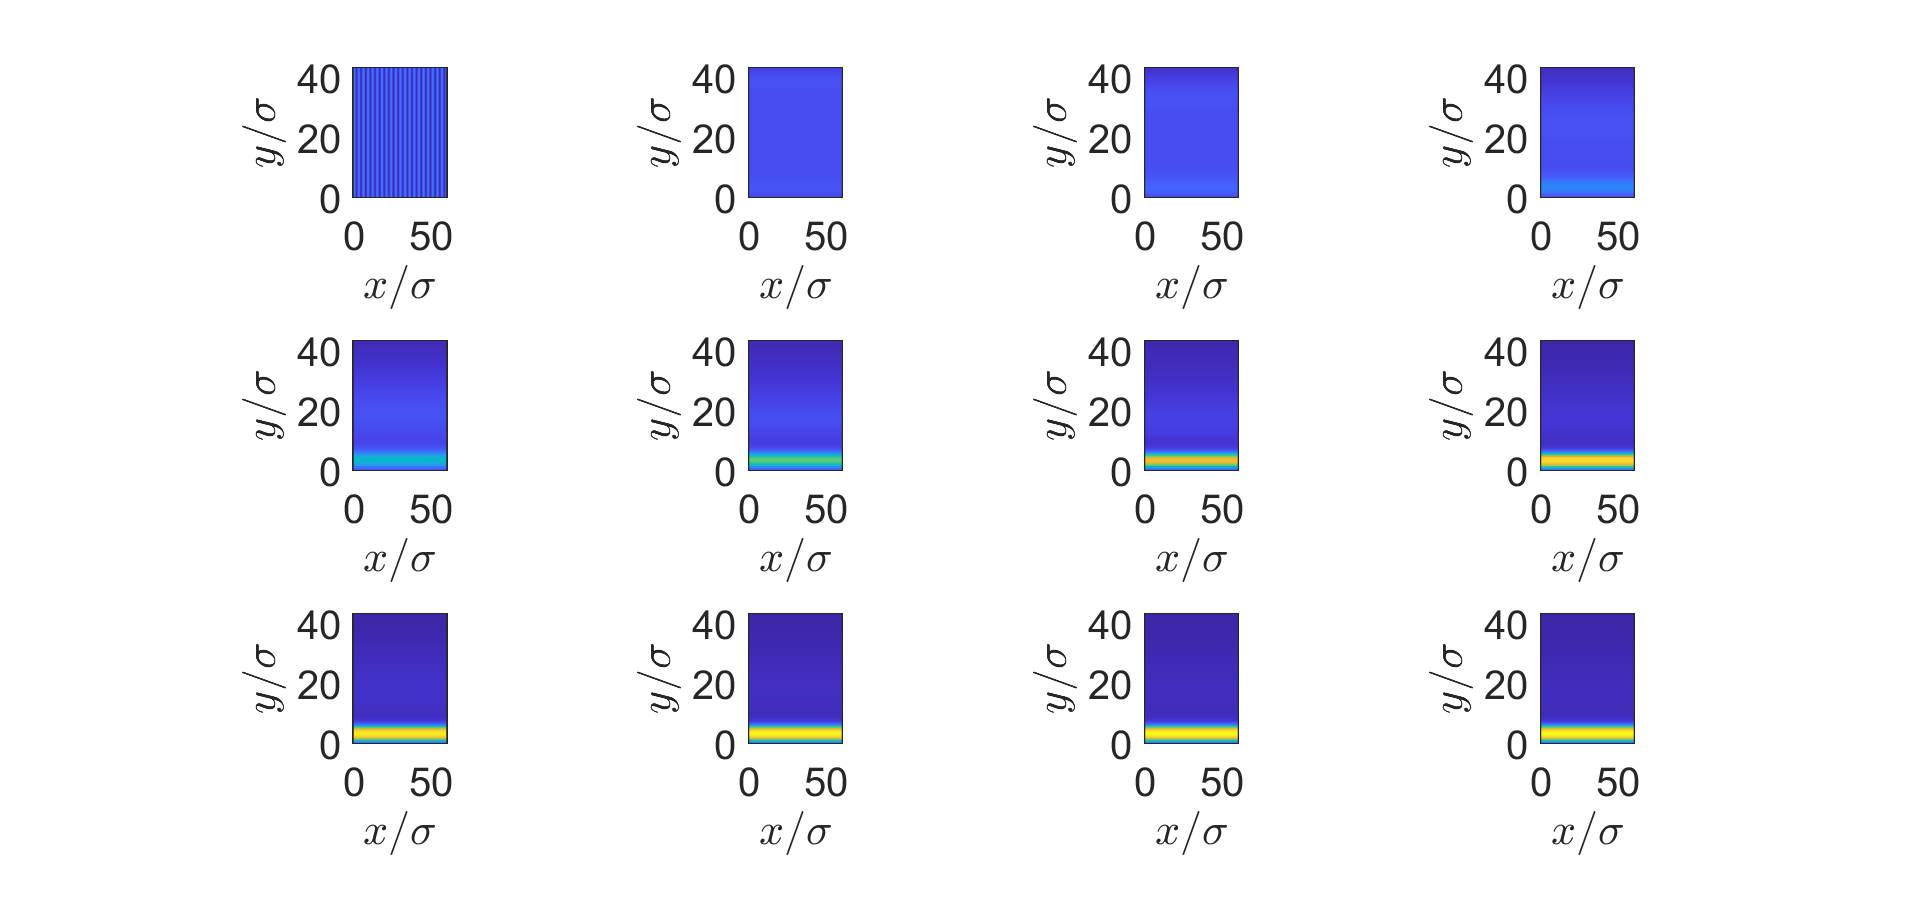
\includegraphics[scale=0.4]{Sed5.png}
	\caption{Figure 8 from paper with $\sigma = 1$, $\bar \rho = 0.072 (\cos(\pi y_2) +1 )$ running up to $t^* = 600$ instead of $t^* = 300$.} 
	\label{F1e}
\end{figure}
\section{Constriction Flow}
I first tried to rewrite the initial condition in terms of $h = 0$. It does solve for a smaller external potential and without constriction, but I still get the warning with the integration tolerances. \\

Then I went back to the original problem. This solves well with $V_0 = 10$ instead of $V_0 = 1000$ and the quality of the result becomes worse for higher strengths of the external potential. 
With this I could put the interaction on. However, they are influenced by the boundaries. Therefore, I put the problem into periodic boundaries. This works but it's not comparable to the results from the paper.
\begin{figure}[h]
	\centering
	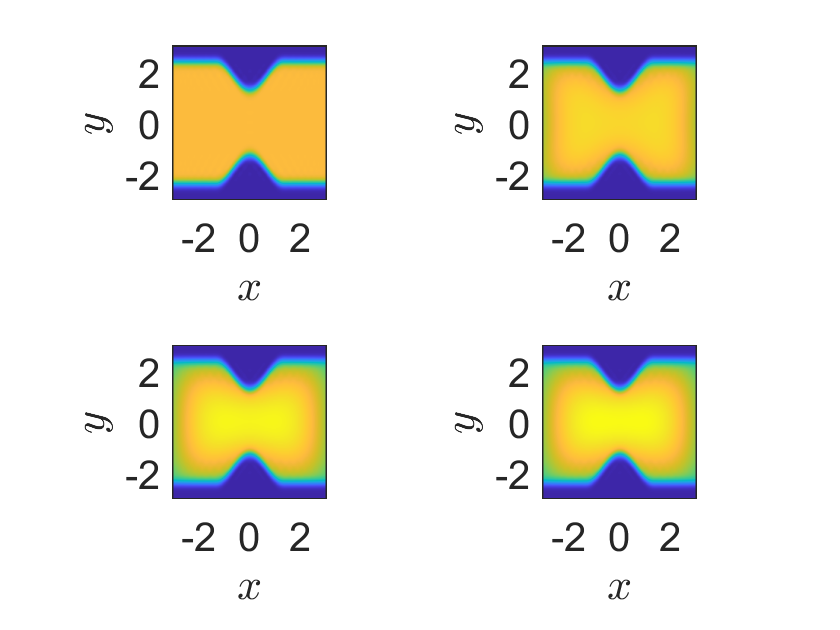
\includegraphics[scale=0.6]{Con1.png}
	\caption{Constriction with $\kappa = -0.2$ and $b = 0.6$, $V_0 = 10$.} 
	\label{F2}
\end{figure}

\begin{figure}[h]
	\centering
	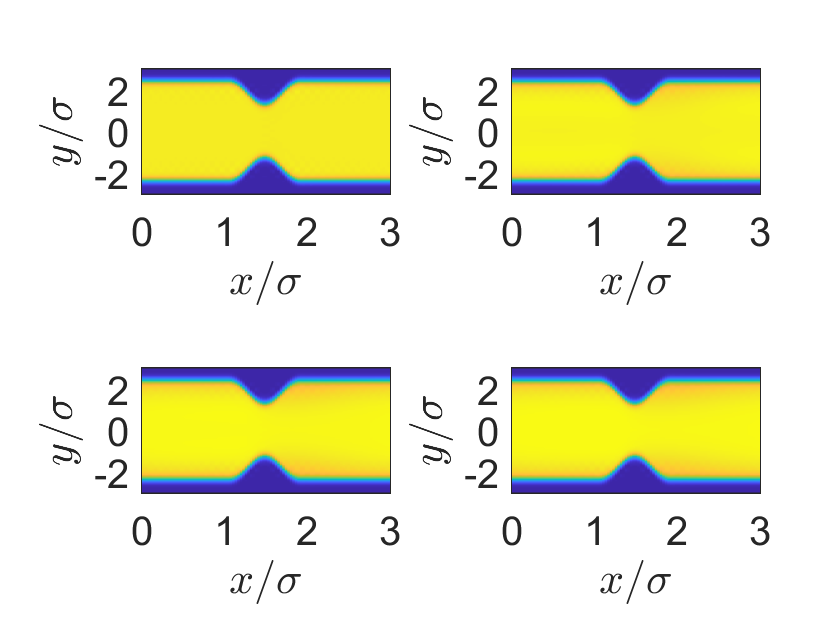
\includegraphics[scale=0.6]{Con2.png}
	\caption{Constriction with $\kappa = -0.2$ and $b = 0.6$, $V_0 = 10$.} 
	\label{F3}
\end{figure}


\begin{figure}[h]
	\centering
	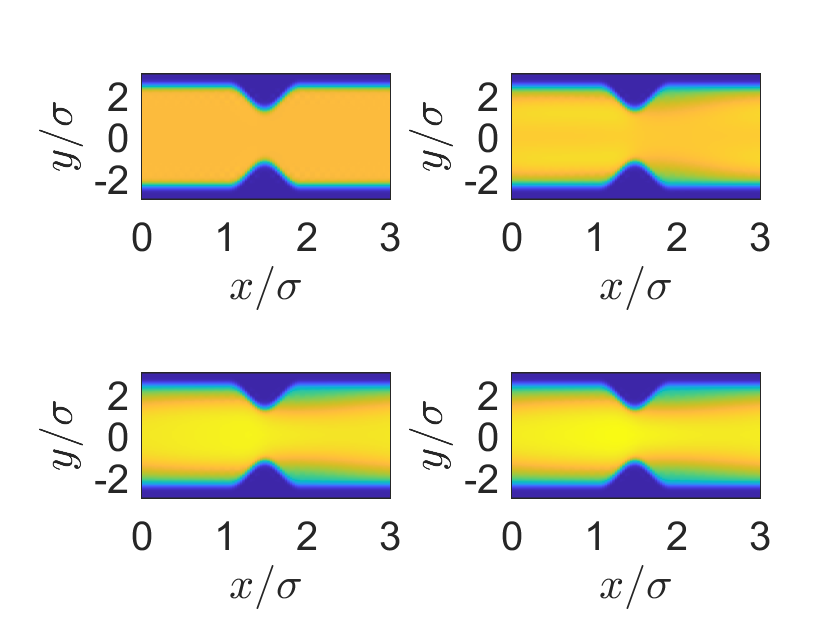
\includegraphics[scale=0.6]{Con3.png}
	\caption{Constriction with $\kappa = -0.6$ and $b = 0.6$, $V_0 = 10$.} 
	\label{F4}
\end{figure}


\begin{figure}[h]
	\centering
	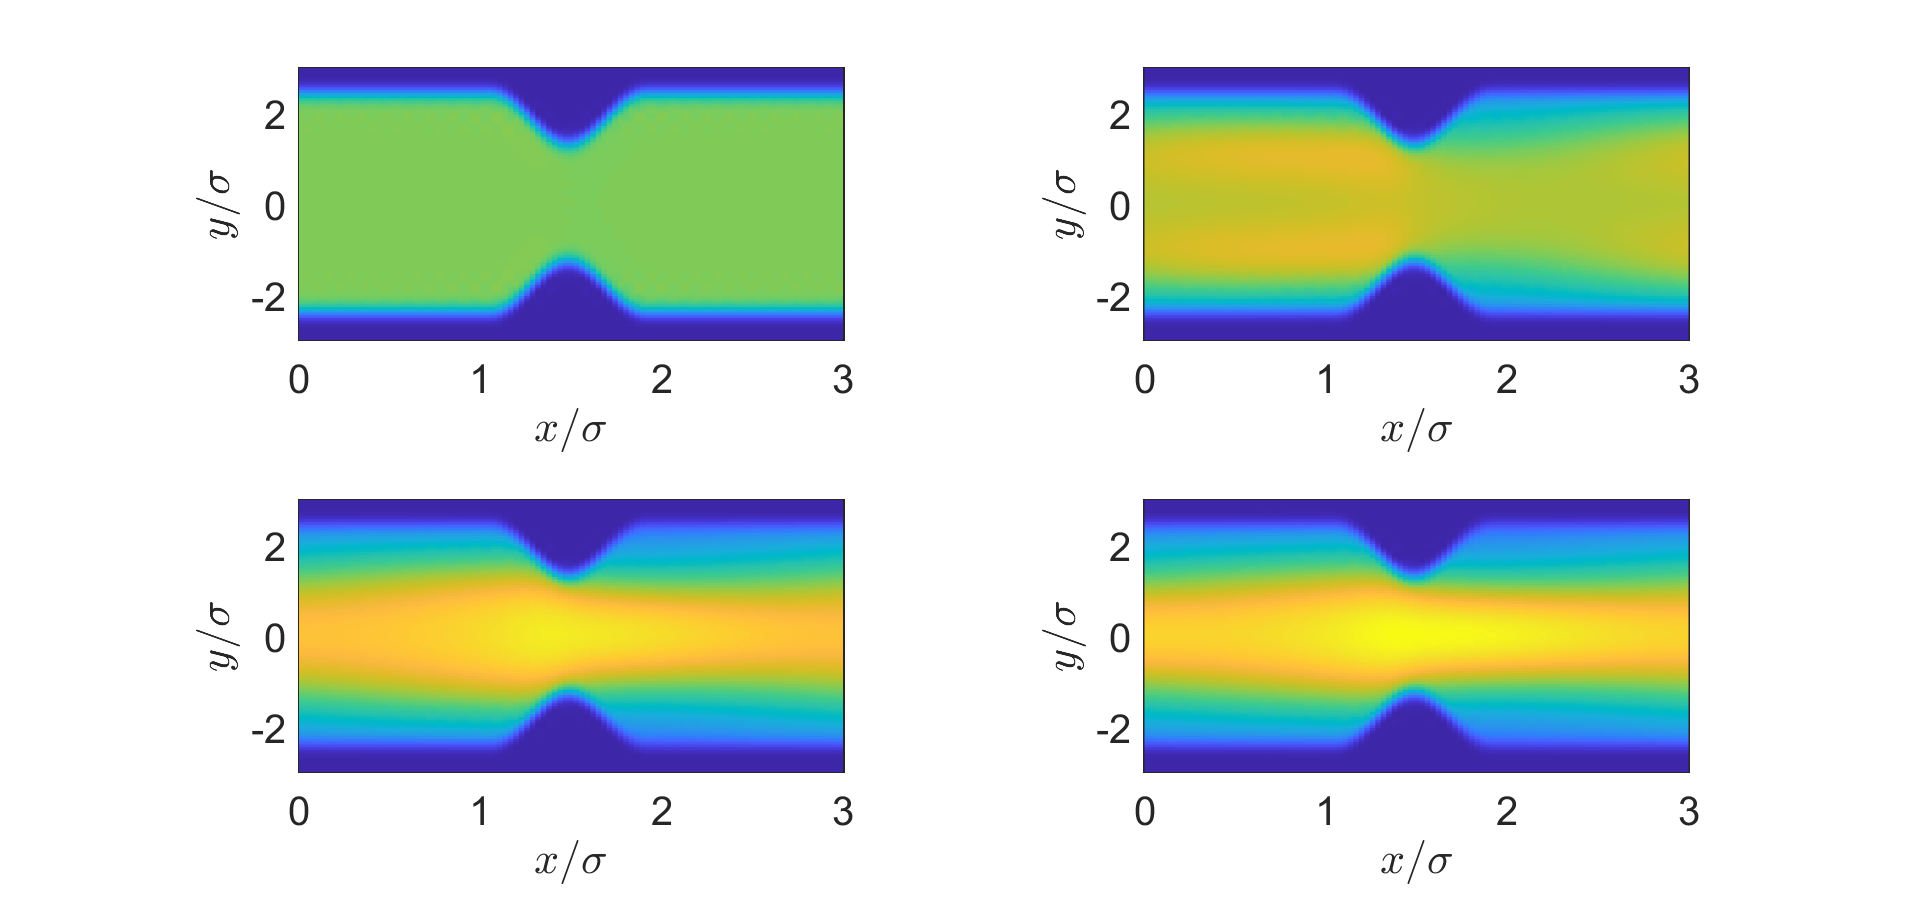
\includegraphics[scale=0.3]{Con4.png}
	\caption{Constriction with $\kappa = -1$ and $b = 0.6$, $V_0 = 10$.} 
	\label{F5}
\end{figure}





















\end{document}